\documentclass[12pt, a4paper]{article}

\usepackage{amsmath, amsthm, amssymb}
\usepackage{geometry}
\usepackage{graphicx}
\usepackage{float}
\usepackage{hyperref}
\usepackage{booktabs}
\usepackage{caption}

\geometry{margin=1in}

\newtheorem{theorem}{Theorem}
\newtheorem{lemma}{Lemma}
\newtheorem{proposition}{Proposition}
\newtheorem{assumption}{Assumption}
\newtheorem{remark}{Remark}

\title{Resilient I-Bug Navigation under Intermittent Signal Spoofing}
\author{
  Tsuriel Vizel \and Avraham Guez \\[1ex]
  \small Supervisor: Dr.\ Andrey Zhitnikov \\
  \small Technion -- Israel Institute of Technology
}
\date{\today}

\begin{document}

\maketitle

\begin{abstract}
Sensor-based bug algorithms provide provable navigation guarantees under a minimalist sensing paradigm. However, algorithms relying exclusively on scalar signal intensity, such as the I-Bug algorithm, are acute targets for adversarial spoofing. In many noncoherent sensing settings, the receiver observes additive intensity contributions from multiple emitters rather than winner-take-all replacement. When a malicious transmitter broadcasts intermittent spoofing signals under an incoherent additive received-signal-strength (RSS) model, these emissions superimpose onto the legitimate target field, distorting both the spatial intensity gradient and the boundary extrema that govern obstacle-departure decisions. This paper introduces an anomaly-detecting extension to the I-Bug framework designed to preserve target convergence in the presence of an intermittent additive adversary without requiring additional hardware, odometry, or global localization. By exploiting the separation of timescales between kinematically bounded spatial intensity variations and step-like temporal discontinuities, our filter reliably isolates spoofing transitions. We formulate and evaluate three behavioral strategies: the unmodified \textit{Naive} I-Bug baseline, a \textit{Cautious} strategy that conditionally preserves the convergence guarantee of benign I-Bug under Assumptions~1--2, and an open-loop \textit{Inertial} heuristic. We prove mathematically that under intermittent step-spoofing (Assumptions~1--2), the Cautious strategy preserves the exact active-state spatial trace of the corresponding benign I-Bug execution. To empirically evaluate our theoretical analysis, we developed a continuous 2D kinematic simulation in Julia and tested all three strategies across $1,000,000$ procedurally generated obstacle environments. Under the sampled environment distribution, while the Naive baseline succeeds in only $54.68\% \pm 0.10\%$ of scenarios, the fast Inertial heuristic achieves a $99.61\% \pm 0.01\%$ success rate (reducing mean completion steps among successful runs by $20.5\%$ and unconditional horizon-capped steps by $16.8\%$ relative to Cautious, while failing in $0.39\%$ of trials), and the Cautious strategy achieves a $100.00\%$ observed success rate ($95\%$ Clopper--Pearson CI: $[99.9996\%, 100.00\%]$), matching the no-attack I-Bug reference and eliminating spoofing-induced failures under the assumed threat model.
\end{abstract}

\section{Introduction}
Autonomous navigation in unknown, GPS-denied environments remains a central problem in mobile robotics. Bug algorithms address this challenge through a minimalist sensing paradigm, enabling a mobile agent to navigate toward a target using strictly local sensory feedback without global maps or absolute localization \cite{lumelsky1987path}. Over the past three decades, numerous extensions have incorporated range sensors to shorten paths, such as TangentBug \cite{kamon1998tangentbug}. At the extreme end of sensory minimalism, the I-Bug algorithm—introduced by Taylor and LaValle at ICRA 2009 \cite{taylor2009ibug} and later expanded with complete convergence proofs and hardware validation \cite{taylor2014intensity}—requires only a binary contact sensor and a scalar signal-intensity sensor measuring emission strength from a target beacon, eliminating the need for spatial coordinates or wheel odometry.

While the classical I-Bug algorithm is mathematically sound under benign conditions, its convergence proof relies on a fragile premise: that the target beacon is the sole source of signal intensity in the workspace. In contested or hostile environments, an adversary may deploy a spoofing transmitter to disrupt navigation \cite{psiaki2016gnss, kerns2014unmanned}. In many noncoherent power-sensing modalities (such as wideband RF RSS, noncoherent optical photodetection, or acoustic energy integration), concurrent emissions do not follow winner-take-all replacement. We therefore study an incoherent additive RSS abstraction in which adversarial and legitimate source contributions are summed at the receiver. This additive interference warps the spatial gradient vector field in free space and induces false local maxima along obstacle boundaries, causing standard intensity-based bug algorithms to deviate from the target or become permanently trapped in infinite boundary-following loops.

This paper addresses this vulnerability by introducing a kinematics-based temporal anomaly filter coupled with state-preserving navigation strategies. To the best of our knowledge, we are not aware of a prior anti-spoofing mechanism designed specifically for the minimalist I-Bug sensing framework. We show that under an intermittent additive spoofing model, a minimalist robot can detect and reject spoofing bursts by analyzing temporal discontinuities in its scalar intensity stream.

\subsection{Related Work}
Our work intersects minimalist bug navigation, physical-layer navigation spoofing, and physics-informed anomaly detection in cyber-physical systems (CPS):
\begin{itemize}
    \item \textbf{Minimalist Bug Navigation:} Classical bug algorithms (\text{Bug1}, \text{Bug2}) rely on contact sensing and odometry to circumnavigate obstacles \cite{lumelsky1987path}, while range-augmented variants such as TangentBug \cite{kamon1998tangentbug} leverage local freespace geometry. Taylor and LaValle's I-Bug \cite{taylor2009ibug, taylor2014intensity} replaces geometric distance with scalar intensity from a single beacon, proving convergence when level sets are non-degenerate, but does not consider adversarial emitters.
    \item \textbf{Navigation and Beacon Spoofing:} Spoofing attacks on autonomous vehicles and unmanned aerial vehicles (UAVs) have been widely studied in the context of GNSS/GPS signals \cite{kerns2014unmanned, psiaki2016gnss} and wireless localization beacons. Existing defenses typically rely on cryptographic authentication, multi-antenna angle-of-arrival arrays, or inertial measurement units (IMUs)—resources unavailable to a strictly minimalist I-Bug agent.
    \item \textbf{Resilient Control and CPS Anomaly Detection:} Secure state estimation and attack detection in CPS have been extensively analyzed using control-theoretic invariants \cite{pasqualetti2013attack, fawzi2014secure, giraldo2018survey} and sequential change-point detection \cite{basseville1993detection}. Our anomaly filter adapts the principle of physics-informed residual checking \cite{giraldo2018survey} to a memory-constrained, coordinate-free bug automaton by bounding legitimate signal variations via the robot's own kinematic velocity limit.
\end{itemize}

\subsection{Contributions and Organization}
The main contributions of this work are threefold:
\begin{enumerate}
    \item \textbf{Additive Spoofing Model \& Kinematic Anomaly Filter:} We formulate the intermittent additive spoofing problem and derive a temporal anomaly detector that distinguishes kinematically bounded spatial intensity changes from adversarial switching discontinuities without oracle access to the true target field.
    \item \textbf{Behavioral Counter-Strategies \& Formal Analysis:} We propose the \textit{Cautious} (state-freezing) and \textit{Inertial} (open-loop continuation) strategies, establish a conditional preservation theorem showing that Cautious preserves the exact active-state spatial path and convergence of any converging benign I-Bug execution under Assumptions~1--2 (Theorem~\ref{thm:cautious_convergence}), and prove that freezing memory alone while continuing deterministic boundary motion is insufficient to guarantee universal convergence due to topological phase-locking (Proposition~\ref{prop:inertial_resonance}).
    \item \textbf{Large-Scale Empirical Evaluation:} We evaluate all three strategies in paired trials across $1,000,000$ randomized, topologically complex 2D environments, quantifying the trade-off between guaranteed convergence and average execution time.
\end{enumerate}

The remainder of this paper is organized as follows. Section~\ref{sec:formulation} formulates the workspace, sensor model, and adversarial superposition field. Section~\ref{sec:algorithm} details the anomaly detection filter and the three navigation strategies. Section~\ref{sec:theory} presents the formal mathematical guarantees and failure-mode analysis. Section~\ref{sec:simulation} describes the kinematic simulation architecture, followed by statistical results and a resonance-trap case study in Section~\ref{sec:results}. Section~\ref{sec:limitations} discusses limitations and future directions, and Section~\ref{sec:conclusion} concludes the paper.

\section{Problem Formulation}
\label{sec:formulation}
Consider a disk-shaped robot of radius $r_c > 0$ (equivalently, a point robot navigating in a configuration space with obstacles inflated by $r_c$) within a bounded planar workspace $\mathcal{W} \subset \mathbb{R}^2$ populated with a finite collection of unknown, piecewise-analytic obstacles $\mathcal{O} = \{O_1, \dots, O_M\}$. Let $\mathcal{F} \subset \mathcal{W}$ denote the collision-free navigable configuration space for the robot center. A target tower located at an unknown fixed position $p_t \in \mathcal{F}$ broadcasts a continuous, isotropic navigation signal. In the absence of interference, the intensity at position $p \in \mathcal{F}$ is given by a strictly decreasing radial function of the Euclidean distance $d(p, p_t) = \|p - p_t\|_2$:
\begin{equation}
    m(p - p_t) = \frac{1}{\|p - p_t\|_2}.
    \label{eq:target_field}
\end{equation}
The mission terminates successfully when the robot enters the target capture radius $\|p - p_t\|_2 < R_{\text{reach}}$.

\subsection{Sensory Paradigm and Motion Primitives}
Following the minimalist I-Bug formulation \cite{taylor2014intensity}, the robot has no access to global coordinates $p$, target coordinates $p_t$, or odometric distance. Its state at discrete control step $k \in \mathbb{N}_0$ (with step period $\Delta t$) consists of its physical pose $q_k = (p_k, \theta_k) \in \mathcal{F} \times [0, 2\pi)$ and its internal navigation memory. The robot is equipped with:
\begin{enumerate}
    \item A local contact/range bumper detecting obstacle boundaries within distance $r_s > r_c$ in the forward and left-lateral sectors;
    \item A scalar intensity sensor measuring the total received signal $S(p_k, t_k)$;
    \item A local gradient-direction estimate obtained from spatially local queries of the same scalar intensity sensor, as assumed by the underlying I-Bug implementation \cite{taylor2014intensity}:
    \begin{equation}
        \theta_{\nabla}(p, t) = \operatorname{atan2}\!\left(\frac{\partial S(p, t)}{\partial y},\, \frac{\partial S(p, t)}{\partial x}\right) \pmod{2\pi}.
        \label{eq:gradient_angle}
    \end{equation}
    This realizes the I-Bug orientation primitive without an additional sensor: in simulation, the partial derivatives are approximated via central finite differences of $S$ at four nearby probe points within one control step (assuming $u(t)$ does not switch during the intra-step probes).
\end{enumerate}

Navigation is executed via three motion primitives over each control step $\Delta t$ with maximum translational step size $\Delta s = v_{\max}\Delta t$:
\begin{itemize}
    \item $u_{\text{ori}}$ (\textbf{Orient to Gradient}): Aligns the robot's heading with the perceived steepest-ascent direction, $\theta_k \leftarrow \theta_{\nabla}(p_k, t_k)$.
    \item $u_{\text{fwd}}$ (\textbf{Move Forward}): Advances the robot linearly along its current heading, $p_{k+1} = p_k + \Delta s \, (\cos\theta_k, \sin\theta_k)^\top$, provided $p_{k+1} \in \mathcal{F}$.
    \item $u_{\text{fol}}$ (\textbf{Follow Obstacle Boundary}): Keeps the contacted obstacle on the robot's left side by scanning candidate headings clockwise from $\theta_k + \pi/2$ in increments of $\Delta\phi$ and advancing by $\Delta s$ along the leftmost collision-free heading that maintains left-bumper proximity (or rotating clockwise in place at inward corners).
\end{itemize}

In standard I-Bug, the robot alternates between two high-level states:
\begin{itemize}
    \item \texttt{MoveToTower}: At each step, the robot aligns with the local gradient via $u_{\text{ori}}$ and steps forward via $u_{\text{fwd}}$. If an obstacle blocks forward motion, the robot records the hit threshold $i_H \leftarrow \max(S(p_k, t_k), i_H)$, turns right by $\pi/2$, and transitions to \texttt{FollowObstacle}.
    \item \texttt{FollowObstacle}: The robot tracks the obstacle perimeter via $u_{\text{fol}}$, recording the local maximum intensity $i_{\text{max}}$ encountered along the boundary. Once the robot has climbed strictly above the hit threshold ($i_{\text{max}} > i_H + \epsilon$) and subsequently detects a descending sample ($S(p_k, t_k) < i_{\text{max}} - \epsilon$), it updates $i_H \leftarrow i_{\text{max}}$, re-orients via $u_{\text{ori}}$, and transitions back to \texttt{MoveToTower}.
\end{itemize}

\subsection{Adversarial Superposition Model}
To disrupt navigation, a stationary adversarial tower located at an unknown position $p_e \in \mathcal{F}$ broadcasts an intermittent spoofing signal of strength $\alpha_e > 0$.

\begin{assumption}[Additive Received-Signal-Strength Superposition]
\label{assump:superposition}
We consider an incoherent additive received-signal-strength (RSS) model in which the sensor reports the sum of the legitimate target intensity and the adversarial emission at position $p \in \mathcal{F}$ and time $t \ge 0$:
\begin{equation}
    S(p, t) = m(p - p_t) + e(p, t), \qquad e(p, t) = u(t)\, m_e(p - p_e) = u(t)\, \frac{\alpha_e}{\|p - p_e\|_2},
    \label{eq:superposition}
\end{equation}
where $u(t) \in \{0, 1\}$ is a piecewise-constant switching function indicating whether the adversary is active at time $t$.
\end{assumption}

Crucially, when $u(t) = 1$, the adversarial component $e(p, t)$ depends on $p$, thereby corrupting \emph{both} the scalar magnitude $S(p, t)$ and its spatial gradient:
\begin{equation}
    \nabla_p S(p, t) = -\frac{p - p_t}{\|p - p_t\|_2^3} - u(t)\,\alpha_e \frac{p - p_e}{\|p - p_e\|_2^3}.
    \label{eq:corrupted_gradient}
\end{equation}
Consequently, an unprotected robot executing $u_{\text{ori}}$ in \texttt{MoveToTower} is deflected toward the vector sum of both towers, while a robot in \texttt{FollowObstacle} records artificially inflated hit/peak intensities $i_H$ that cannot be exceeded once $u(t)$ reverts to $0$, permanently trapping the robot on the obstacle boundary.

\begin{assumption}[Temporal Discontinuity vs.\ Kinematically Bounded Spatial Variation]
\label{assump:discontinuity}
The robot's translational velocity is bounded by $v_{\max}$, and the sensor samples intensity across a high-rate temporal window $\delta t \ll \Delta t$ corresponding to a maximum spatial displacement $\delta s = v_{\max}\delta t \ll R_{\text{reach}}$. Over any time interval $[t - \delta t, t]$ during which the adversary is inactive ($u \equiv 0$), the variation in intensity due to robot motion from reference intensity $I_{\text{ref}} = m(p - p_t) = 1/d$ is bounded by the local radial Lipschitz increment:
\begin{equation}
    \bigl|m(p(t) - p_t) - m(p(t - \delta t) - p_t)\bigr| \le \Delta I_{\max}(I_{\text{ref}}) = \frac{\delta s}{d(d - \delta s)} = \frac{\delta s\, I_{\text{ref}}^2}{1 - \delta s\, I_{\text{ref}}}.
    \label{eq:lipschitz_bound}
\end{equation}
Conversely, the adversary switches $u(t)$ between $0$ and $1$ as a discrete step function such that every active burst lasts at most $T_{\text{on}} \ge 1$ steps and every inactive interval lasts at least $T_{\text{off}} > N_{\text{confirm}}$ steps (after an initial delay $T_{\text{delay}}$; a fixed-period schedule is a special case). Let $\mathcal{F}_{\text{nav}} = \{p \in \mathcal{F} : \|p - p_t\|_2 \ge R_{\text{reach}}\}$. At any switching instant $t$, the minimum instantaneous jump across the navigable workspace,
\begin{equation}
    e_{\min} := \min_{p \in \mathcal{F}_{\text{nav}}} m_e(p - p_e) = \frac{\alpha_e}{\max_{p \in \mathcal{F}_{\text{nav}}} \|p - p_e\|_2} \ge \frac{\alpha_e}{\operatorname{diam}(\mathcal{W})},
    \label{eq:emin_def}
\end{equation}
satisfies the separability condition:
\begin{equation}
    e_{\min} > \eta_{\text{spike}} \max_{p \in \mathcal{F}_{\text{nav}}} \Delta I_{\max}\!\bigl(m(p - p_t)\bigr),
    \label{eq:detectability_condition}
\end{equation}
where $\eta_{\text{spike}} > 1$ is the spike anomaly threshold multiplier.
\end{assumption}

\begin{remark}[Physical Motivation, Scope, and Bounded-Noise Conditions]
\label{rem:physical_justification}
Assumption~\ref{assump:discontinuity} is physically motivated by time-scale separation: electronic intensity sampling ($\text{kHz}$ rate) is orders of magnitude faster than mechanical robot translation ($v_{\max}$), making $\delta s = v_{\max}\delta t$ and $\Delta I_{\max}$ small relative to abrupt switching transients. The guarantee excludes continuously active, slowly ramped (adiabatic), or sufficiently weak attacks whose temporal residual remains below the detection threshold \cite{psiaki2016gnss}; formal characterization of such stealthy or near-field attacks (where $\alpha_e / \|p - p_e\|_2$ remains below threshold while $\|\nabla e(p)\| = \alpha_e / \|p - p_e\|_2^2$ noticeably perturbs the gradient direction) is left for future work. In particular, a defense-aware adversary can stall the Cautious robot indefinitely (denial of service) by keeping $u(t) = 1$ or switching off for at most $N_{\text{confirm}}$ steps; Theorem~\ref{thm:cautious_convergence} guarantees safety, not liveness, against such attackers. Finally, under bounded measurement noise $|\nu_k| \le \varepsilon_{\text{noise}}$ (so $|\nu_k - \nu_{k-1}| \le 2\varepsilon_{\text{noise}}$), false-positive spike detections are excluded if $\Delta I_{\max} + 2\varepsilon_{\text{noise}} < \eta_{\text{spike}}\Delta I_{\max}$, while activation events remain guaranteed to trigger $\mathcal{A}_{\text{spike}}$ (no false negatives) if $e_{\min} - 2\varepsilon_{\text{noise}} > \eta_{\text{spike}}\Delta I_{\max}$. Analogously, for the deactivation detector $\mathcal{A}_{\text{drop}}$ with multiplier $\eta_{\text{drop}} \in (1, \eta_{\text{spike}}]$, false positives and false negatives are excluded under $\Delta I_{\max} + 2\varepsilon_{\text{noise}} < \eta_{\text{drop}}\Delta I_{\max}$ and $e_{\min} - 2\varepsilon_{\text{noise}} > \eta_{\text{drop}}\Delta I_{\max}$, respectively.
\end{remark}

\section{The Proposed Anti-Adversary Framework}
\label{sec:algorithm}
Motivated by physics-based attack detection \cite{giraldo2018survey} and classical abrupt-change detection \cite{basseville1993detection}, to protect navigation without additional sensors or oracle knowledge of $m(p - p_t)$, we interpose a temporal anomaly detection filter between the intensity sensor and the I-Bug state machine.

\subsection{Temporal Anomaly Detection Filter}
At the beginning of each control step $k$, prior to executing spatial actuation, the robot samples the current perceived intensity $I_k^- = S(p_{k-1}, t_k)$ and compares it against the post-actuation intensity recorded at the conclusion of step $k-1$, $I_{k-1}^+ = S(p_{k-1}, t_{k-1})$. Let $\Delta I_k = I_k^- - I_{k-1}^+$ denote the temporal intensity variation across the step boundary, and let $\Delta I_{\max}(I)$ be defined by Eq.~\eqref{eq:lipschitz_bound}. We define two boolean anomaly detectors:
\begin{enumerate}
    \item \textbf{Positive (Spike) Anomaly ($\mathcal{A}_{\text{spike}}$):} Flagged when the intensity exhibits an unphysical upward jump relative to the pre-transition reference $I_{k-1}^+$ (which equals the uncorrupted target signal $m(p_{k-1}-p_t) = 1/d$ whenever a transition $0 \to 1$ occurs):
    \begin{equation}
        \mathcal{A}_{\text{spike}}(I_k^-, I_{k-1}^+) \iff \Delta I_k > \eta_{\text{spike}} \cdot \Delta I_{\max}(I_{k-1}^+),
        \label{eq:spike_detector}
    \end{equation}
    with $\eta_{\text{spike}} = 2.0$.
    \item \textbf{Negative (Drop) Anomaly ($\mathcal{A}_{\text{drop}}$):} Flagged when the intensity exhibits an unphysical downward drop corresponding to adversary deactivation ($1 \to 0$, where the post-transition reading $I_k^- = m(p_{k-1}-p_t) = 1/d$ is again uncorrupted):
    \begin{equation}
        \mathcal{A}_{\text{drop}}(I_k^-, I_{k-1}^+) \iff (-\Delta I_k > 0.15\, I_{k-1}^+) \;\lor\; \bigl(-\Delta I_k > \eta_{\text{drop}} \cdot \Delta I_{\max}(I_k^-)\bigr),
        \label{eq:drop_detector}
    \end{equation}
    with $\eta_{\text{drop}} = 1.2$.
\end{enumerate}

Both $I_k^-$ and $I_{k-1}^+$ are evaluated at the same position $p_{k-1}$, so the benign variation $\Delta I_k$ is identically zero in our noiseless discrete-time simulation; $\Delta I_{\max}$ provides a conservative physical margin for sensors that integrate over $\delta t$ while moving up to $\delta s$, and for bounded measurement noise (Remark~\ref{rem:physical_justification}). The $15\%$ relative drop clause in Eq.~\eqref{eq:drop_detector} is a heuristic safeguard that only adds detections and is not relied upon in the formal analysis. Crucially, at no point does any strategy access $m(p - p_t)$ or $p_t$ directly; all orientation ($u_{\text{ori}}$) and boundary-following decisions operate exclusively on $S(p, t)$.

\subsection{Strategy 1: The Naive Strategy (Original I-Bug Baseline)}
The \textit{Naive} strategy represents the unmodified baseline I-Bug algorithm of Taylor and LaValle \cite{taylor2014intensity}, in which the anomaly filter is absent. At every step $k$:
\begin{itemize}
    \item In \texttt{MoveToTower}, the robot orients along the perceived gradient $\theta_{\nabla}(p_k, t_k)$ via $u_{\text{ori}}$ and advances via $u_{\text{fwd}}$. When the adversary is active ($u(t_k)=1$), $\theta_{\nabla}$ points along the corrupted superposition field in Eq.~\eqref{eq:corrupted_gradient}, deflecting the robot away from the true target path.
    \item Upon hitting an obstacle or following its boundary in \texttt{FollowObstacle}, the robot updates $i_H$, $i_{\text{max}}$, and its global memory $i_{\text{mem}}$ using the raw superimposed reading $S(p_k, t_k)$.
\end{itemize}

\subsection{Strategy 2: The Cautious Strategy}
The \textit{Cautious} strategy prioritizes strict state preservation and provable convergence:
\begin{itemize}
    \item \textbf{Normal Mode:} While in \texttt{Normal} mode, if $\mathcal{A}_{\text{spike}}(I_k^-, I_{k-1}^+)$ triggers, the robot immediately transitions to \texttt{Paused} mode, locks its pose $(p_{\text{frozen}}, \theta_{\text{frozen}}) \leftarrow (p_{k-1}, \theta_{k-1})$ and navigation state (\texttt{MoveToTower} or \texttt{FollowObstacle}), sets the confirmation counter $c \leftarrow 0$, and executes zero motion ($\Delta p_k = 0$) without modifying $i_H$, $i_{\text{max}}$, or $i_{\text{mem}}$. Otherwise, it executes a standard I-Bug step using $S(p, t_k)$.
    \item \textbf{Paused Mode:} While \texttt{Paused}, the robot remains stationary ($\Delta p_k = 0$) and ignores all boundary and memory updates. When $\mathcal{A}_{\text{drop}}(I_k^-, I_{k-1}^+)$ is detected, it initializes the confirmation counter $c \leftarrow 1$. Over subsequent steps, if another spike occurs, $c$ resets to $0$; otherwise $c$ increments by $1$ each step. Once $c = N_{\text{confirm}}$ (with $N_{\text{confirm}} = 3$), the environment is confirmed clear, the robot restores its frozen state and heading, transitions back to \texttt{Normal} mode, and resumes navigation on the next step.
\end{itemize}

\subsection{Strategy 3: The Inertial Strategy (Heuristic)}
The \textit{Inertial} strategy seeks to convert spoofed intervals into productive forward progress via open-loop continuation:
\begin{itemize}
    \item \textbf{Transition to Inertial Mode:} When $\mathcal{A}_{\text{spike}}(I_k^-, I_{k-1}^+)$ triggers during \texttt{Normal} mode, the robot transitions to \texttt{InertialMode}, freezes its current heading $\theta_{\text{frozen}} \leftarrow \theta_{k-1}$, suspends all updates to $i_{\text{mem}}$ and $i_{\text{max}}$, and immediately executes one open-loop inertial step.
    \item \textbf{Open-Loop Execution:} During \texttt{InertialMode}:
    \begin{enumerate}
        \item If the robot is in \texttt{MoveToTower}, it \emph{suppresses} $u_{\text{ori}}$ (keeping $\theta_k = \theta_{\text{frozen}}$) and steps forward linearly via $u_{\text{fwd}}$. If it contacts an obstacle while blind, it cannot trust the corrupted sensor reading $S(p_k, t_k)$; instead, it initializes the obstacle hit threshold using its last valid pre-spoofing memory, $i_H \leftarrow i_{\text{mem}}$, turns right by $\pi/2$, and enters \texttt{FollowObstacle}.
        \item If the robot is in \texttt{FollowObstacle}, it continues physical perimeter traversal via $u_{\text{fol}}$ using its contact sensors, but completely suspends peak updates and the leave-obstacle condition.
    \end{enumerate}
    \item \textbf{Return to Normal Mode:} While in \texttt{InertialMode}, as soon as $\mathcal{A}_{\text{drop}}(I_k^-, I_{k-1}^+)$ triggers, the robot immediately transitions back to \texttt{Normal} mode, updates $i_{\text{mem}} \leftarrow \max(i_{\text{mem}}, I_k^-)$, and resumes closed-loop I-Bug navigation from its new physical position.
\end{itemize}

\section{Mathematical Guarantees and Failure Analysis}
\label{sec:theory}

We first establish a conditional trajectory- and convergence-preservation theorem: whenever the corresponding benign baseline execution reaches the target in $N_{\text{ideal}} < \infty$ active steps, the Cautious strategy produces the exact same sequence of active states and reaches the target after inserting only a finite number of paused steps. Consequently, in environments satisfying the original I-Bug convergence assumptions \cite{taylor2014intensity}, Cautious inherits that guarantee.

\begin{theorem}[Conditional Active-State Trajectory and Convergence Preservation]
\label{thm:cautious_convergence}
Suppose Assumptions~\ref{assump:superposition} and~\ref{assump:discontinuity} hold with $\eta_{\text{drop}} \le \eta_{\text{spike}}$ and $T_{\text{off}} > N_{\text{confirm}}$. Then, for any workspace $\mathcal{W}$ and benign intensity field $m$:
\begin{enumerate}
    \item After removing the paused steps, the ordered sequence of spatial poses $\gamma_{\text{cautious}}$ and internal navigation states visited by the Cautious robot coincides step-by-step with the trajectory $\gamma_{\text{ideal}}$ produced by the baseline I-Bug execution in a benign environment ($e(p, t) \equiv 0$).
    \item Whenever the benign baseline execution reaches the target neighborhood $\|p_k - p_t\|_2 < R_{\text{reach}}$ in a finite number of steps $N_{\text{ideal}} < \infty$ (in particular, for any environment satisfying the convergence assumptions of \cite{taylor2014intensity}), the Cautious robot is guaranteed to reach the same target state in a finite number of total steps $N_{\text{cautious}}$, bounded by
    \begin{equation}
        N_{\text{cautious}} \le N_{\text{ideal}} + \left\lceil \frac{N_{\text{ideal}}}{T_{\text{clear}}} \right\rceil \bigl(T_{\text{on}} + N_{\text{confirm}}\bigr),
        \label{eq:step_bound}
    \end{equation}
    where $T_{\text{clear}} = T_{\text{off}} - N_{\text{confirm}} \ge 1$ is the minimum number of effective navigation steps per adversarial switching cycle.
\end{enumerate}
\end{theorem}

\begin{proof}
Let $\mathcal{K}_{\text{spoof}} = \{k \in \mathbb{N} : u(t_k) = 1\}$ denote the set of steps during which the adversary is active, partitioned into contiguous bursts $[k_j^{\text{on}},\, k_j^{\text{off}} - 1]$ for $j = 1, 2, \dots$, where $u(t)$ transitions $0 \to 1$ at step $k_j^{\text{on}}$ and $1 \to 0$ at step $k_j^{\text{off}}$.

\textbf{Step 1 (Soundness and Completeness of Anomaly Switching):}
During any step $k$ where $u(t_k) = u(t_{k-1})$, both $I_{k-1}^+ = S(p_{k-1}, t_{k-1})$ and $I_k^- = S(p_{k-1}, t_k)$ are evaluated at the same spatial configuration $p_{k-1}$ with identical adversary state, yielding $\Delta I_k = 0$ (or bounded by $\Delta I_{\max}(I_{k-1}^+) < \eta_{\text{spike}}\Delta I_{\max}(I_{k-1}^+)$ over sensor sampling displacement $\delta s$). Thus, no false-positive spike or drop anomaly can occur when $u(t)$ is constant.

At each activation step $k = k_j^{\text{on}}$, $u(t_{k-1}) = 0$ and $u(t_k) = 1$, so the temporal jump is
\begin{equation*}
    \Delta I_k = S(p_{k-1}, t_k) - S(p_{k-1}, t_{k-1}) = m_e(p_{k-1} - p_e) \ge e_{\min}.
\end{equation*}
By the detectability condition in Assumption~\ref{assump:discontinuity} (Eq.~\eqref{eq:detectability_condition}), $\Delta I_k \ge e_{\min} > \eta_{\text{spike}}\Delta I_{\max}(I_{k-1}^+)$, so $\mathcal{A}_{\text{spike}}$ triggers immediately at $k_j^{\text{on}}$ before any spatial movement or memory update occurs. The robot enters \texttt{Paused} mode and locks its complete state $\Sigma_{k_j^{\text{on}}-1} = (p_{k_j^{\text{on}}-1}, \theta_{k_j^{\text{on}}-1}, \text{mode}, i_H, i_{\text{max}}, i_{\text{mem}})$.

Throughout $k \in \{k_j^{\text{on}} + 1, \dots, k_j^{\text{off}} - 1\}$, the robot remains stationary ($p_k = p_{k_j^{\text{on}}-1}$) and $u(t_k) = 1$, so $\Delta I_k = 0$ and the robot remains in \texttt{Paused} mode. At the deactivation step $k = k_j^{\text{off}}$, $u(t)$ drops from $1$ to $0$. Since $\eta_{\text{drop}} \le \eta_{\text{spike}}$ and $I_{k_j^{\text{off}}}^- = m(p_{k_j^{\text{on}}-1} - p_t)$, Eq.~\eqref{eq:detectability_condition} also implies the drop-separation inequality:
\begin{equation*}
    -\Delta I_{k_j^{\text{off}}} = m_e(p_{k_j^{\text{on}}-1} - p_e) \ge e_{\min} > \eta_{\text{spike}}\Delta I_{\max}(I_{k_j^{\text{off}}}^-) \ge \eta_{\text{drop}}\Delta I_{\max}(I_{k_j^{\text{off}}}^-),
\end{equation*}
which triggers $\mathcal{A}_{\text{drop}}$ and sets $c = 1$. Since $T_{\text{off}} > N_{\text{confirm}}$, $u(t_k) = 0$ for the next $N_{\text{confirm}} - 1$ stationary steps, incrementing $c$ to $N_{\text{confirm}}$ at step $k_j^{\text{res}} = k_j^{\text{off}} + N_{\text{confirm}} - 1$, where the robot restores $\Sigma_{k_j^{\text{on}}-1}$ and returns to \texttt{Normal} mode.

\textbf{Step 2 (Bijection onto the Ideal Trajectory):}
Define the effective (active) step index $\tau(k) = \sum_{s=1}^k \mathbb{I}(\text{action}_s \notin \{\texttt{Stopped}, \texttt{Resumed}\})$. Whenever the Cautious robot executes an active step ($\mathbb{I} = 1$), the adversary is strictly inactive ($u(t_k) = 0$). Consequently, the perceived field and its spatial gradient during every active step satisfy
\begin{equation*}
    S(p, t_k) = m(p - p_t), \qquad \nabla_p S(p, t_k) = \nabla_p m(p - p_t).
\end{equation*}
Moreover, because the paused interval $[k_j^{\text{on}}, k_j^{\text{res}}]$ leaves the state tuple $\Sigma$ invariant, $\Sigma(k_j^{\text{res}}) = \Sigma(k_j^{\text{on}} - 1)$. By induction on the effective step index $\tau$, the state $\Sigma$ after $\tau$ active steps is identical to the state $\Sigma_{\text{ideal}}(\tau)$ of the baseline I-Bug algorithm operating in a benign environment. Thus, the spatial trace $\gamma_{\text{cautious}}$ coincides pointwise with $\gamma_{\text{ideal}}$.

\textbf{Step 3 (Conditional Finite-Time Convergence and Step Bound):}
Whenever the benign execution $\gamma_{\text{ideal}}$ reaches $\|p - p_t\|_2 < R_{\text{reach}}$ in $N_{\text{ideal}} < \infty$ active steps (which holds for continuous/idealized environments by Taylor and LaValle \cite{taylor2014intensity}), $\gamma_{\text{cautious}}$ reaches the exact same target state at active step $\tau = N_{\text{ideal}}$. Since each adversarial cycle of length $T_{\text{cycle}}$ contains at most $T_{\text{on}} + N_{\text{confirm}}$ paused/resuming steps and at least $T_{\text{clear}} = T_{\text{cycle}} - T_{\text{on}} - N_{\text{confirm}} \ge 1$ active steps, reaching $N_{\text{ideal}}$ active steps requires at most $\lceil N_{\text{ideal}} / T_{\text{clear}} \rceil$ adversarial bursts, establishing Eq.~\eqref{eq:step_bound}.
\end{proof}

\begin{proposition}[Insufficiency of Memory Freezing Alone Under Topological Resonance]
\label{prop:inertial_resonance}
Freezing internal memory alone while continuing deterministic open-loop boundary motion (as in the Inertial heuristic) is insufficient to preserve a universal convergence guarantee. Specifically, let $O_i \in \mathcal{O}$ be an obstacle with boundary perimeter $L_i$, and let $\mathcal{A}_L \subset \partial O_i$ denote the boundary departure-detection arc over which the leave-event sequence—consisting of threshold crossing ($m(p - p_t) > i_H + \epsilon$), local peak observation ($i_{\max}$), and subsequent descent ($m(p - p_t) < i_{\max} - \epsilon$)—must be evaluated. If the robot traverses $\partial O_i$ in \texttt{FollowObstacle} with effective boundary-following speed $v_{\text{fol}}$ such that the orbital period $T_{\text{orbit}} = L_i / (v_{\text{fol}}\Delta t)$ satisfies an exact phase-synchronization condition with the adversarial period $T_{\text{cycle}}$,
\begin{equation}
    T_{\text{orbit}} = m \, T_{\text{cycle}} \quad \text{for some integer } m \ge 1,
    \label{eq:resonance_cond}
\end{equation}
and the blind arc of length $v_{\text{fol}} T_{\text{on}} \Delta t$ traversed during $[k_j^{\text{on}}, k_j^{\text{off}})$ covers $\mathcal{A}_L$ (or prevents completion of the climb--peak--descent sequence across $\mathcal{A}_L$), the Inertial robot will repeatedly bypass $\mathcal{A}_L$ during \texttt{InertialMode} and remain trapped in an infinite limit cycle around $O_i$. (Near-commensurate periods $T_{\text{orbit}} = m\,T_{\text{cycle}} + \varepsilon_{\text{phase}}$ with small $|\varepsilon_{\text{phase}}| > 0$ may similarly produce prolonged, multi-orbit trapping episodes whose duration scales inversely with $|\varepsilon_{\text{phase}}|$ and increases with the width of the blind arc.)
\end{proposition}

\begin{proof}[Proof Sketch]
During \texttt{InertialMode}, the Inertial robot continues physical boundary traversal via $u_{\text{fol}}$ over $T_{\text{on}}$ steps while suspending evaluation of the leave sequence across $\mathcal{A}_L$. When $\mathcal{A}_L$ is covered by the spatial arc of length $v_{\text{fol}} T_{\text{on}} \Delta t$ swept during the $j$-th adversarial burst, the robot traverses $\mathcal{A}_L$ without recording the peak or transitioning to \texttt{MoveToTower}. When $u(t)$ deactivates at $k_j^{\text{off}}$, the robot is already on the descending side of $\partial O_i$ where $m(p - p_t) \le i_H$, forcing it to complete another full orbit of $\partial O_i$. Because $T_{\text{orbit}} = m \, T_{\text{cycle}}$, the robot arrives at the exact same pre-departure boundary position at step $k_j^{\text{on}} + m\,T_{\text{cycle}} = k_{j+m}^{\text{on}}$, causing the $(j+m)$-th adversarial burst to mask $\mathcal{A}_L$ identically on every subsequent revolution.
\end{proof}

\section{Simulation Setup and Methodology}
\label{sec:simulation}
To empirically evaluate the predicted behavior of Theorem~\ref{thm:cautious_convergence} and illustrate the resonance mechanism of Proposition~\ref{prop:inertial_resonance}, we developed a continuous 2D kinematic simulation environment in the Julia programming language. Unlike grid-world approximations, the simulator resolves continuous Euclidean kinematics, exact circle-rectangle collision geometry, and continuous superposition signal fields.

\subsection{Kinematics, Sensing, and Adversary Parameters}
The workspace is a bounded square arena $\mathcal{W} = [0, 20] \times [0, 20]$. All robots initialize at $p_0 = (2.0, 1.0)$ and navigate toward the target tower at $p_t = (18.0, 18.0)$ with capture radius $R_{\text{reach}} = 0.5$. The disk robot has collision radius $r_c = 0.3$, step size $\Delta s = 0.3$, sensor probe range $r_s = 1.1\,r_c$, boundary-following angular resolution $\Delta\phi = 5^\circ$, and anomaly filter sampling displacement $\delta s = 0.002$. Local gradient orientation $u_{\text{ori}}$ is computed via central finite differences of $S(p, t)$ (Eq.~\eqref{eq:gradient_angle}) with probe offset $\varepsilon = 10^{-5}$; this finite-difference calculation emulates local scalar measurements at nearby probe positions and does not expose $p_t$, $p_e$, or their coordinates to the navigation policy.

After an initial delay of $T_{\text{delay}} = 20$ steps, the adversarial tower (with strength $\alpha_e = 1.0$) operates on a $25\%$ duty cycle with period $T_{\text{cycle}} = 40$ steps ($T_{\text{on}} = 10$ active steps followed by $T_{\text{off}} = 30$ inactive steps). For each generated environment, the three strategies (\textit{Naive}, \textit{Cautious}, and \textit{Inertial}) are executed in paired trials under identical obstacle layouts and adversarial placement $p_e$, alongside a no-attack ($u(t) \equiv 0$) benign I-Bug reference execution on the exact same mazes, with a maximum horizon of $N_{\max} = 2,000$ steps.

\subsection{Procedural Topological Environment Generation}
To generate geometrically navigable environments with wide collision-free passages and non-trivial obstacle topologies, each environment is populated with $M \in \{10, \dots, 16\}$ randomly generated horizontal and vertical rectangular walls (length $\in [3.0, 7.0]$, thickness $\in [0.8, 1.6]$). Individual rectangles are permitted to overlap and merge to form non-convex obstacles, U-shaped pockets, and long corridors. Geometric navigability is promoted by enforcing four constraints during rejection sampling:
\begin{enumerate}
    \item \textbf{Clearance Around Start and Target:} A $2.0$-unit obstacle-free buffer is enforced around both $p_0$ and $p_t$.
    \item \textbf{Narrow Gap Prevention:} Any candidate rectangle whose minimum Euclidean distance to an existing disjoint rectangle falls in $(0, 0.8)$ is rejected (since $0.8 > 2r_c = 0.6$), eliminating impassable pinch-points while allowing exact overlaps ($\text{dist} = 0$) to form composite non-convex shapes.
    \item \textbf{Perimeter Margin:} All obstacles are restricted to the interior $[1.0, 19.0]^2$, guaranteeing a continuous navigable corridor of width $1.0 > 2r_c$ along the outer boundary of $\mathcal{W}$.
    \item \textbf{Adversary Placement:} The adversarial tower $p_e$ is sampled uniformly in $\mathcal{F}$ subject to $\|p_e - p_0\|_2 > 6.0$ and $\|p_e - p_t\|_2 > 8.0$.
\end{enumerate}
(Collision-free connectivity between $p_0$ and $p_t$ across all $1,000,000$ generated instances is further witnessed a posteriori by the $100.00\%$ target reachability of the collision-free Cautious trajectory in Section~\ref{sec:results}.)

\section{Statistical Results and Discussion}
\label{sec:results}
We executed $1,000,000$ paired simulations across randomized environments. In each trial, a strategy was recorded as successful if it reached $\|p_k - p_t\|_2 < R_{\text{reach}}$ within $N_{\max} = 2,000$ steps.

\subsection{Convergence Reliability and Temporal Efficiency}

\begin{figure}[htbp]
    \centering
    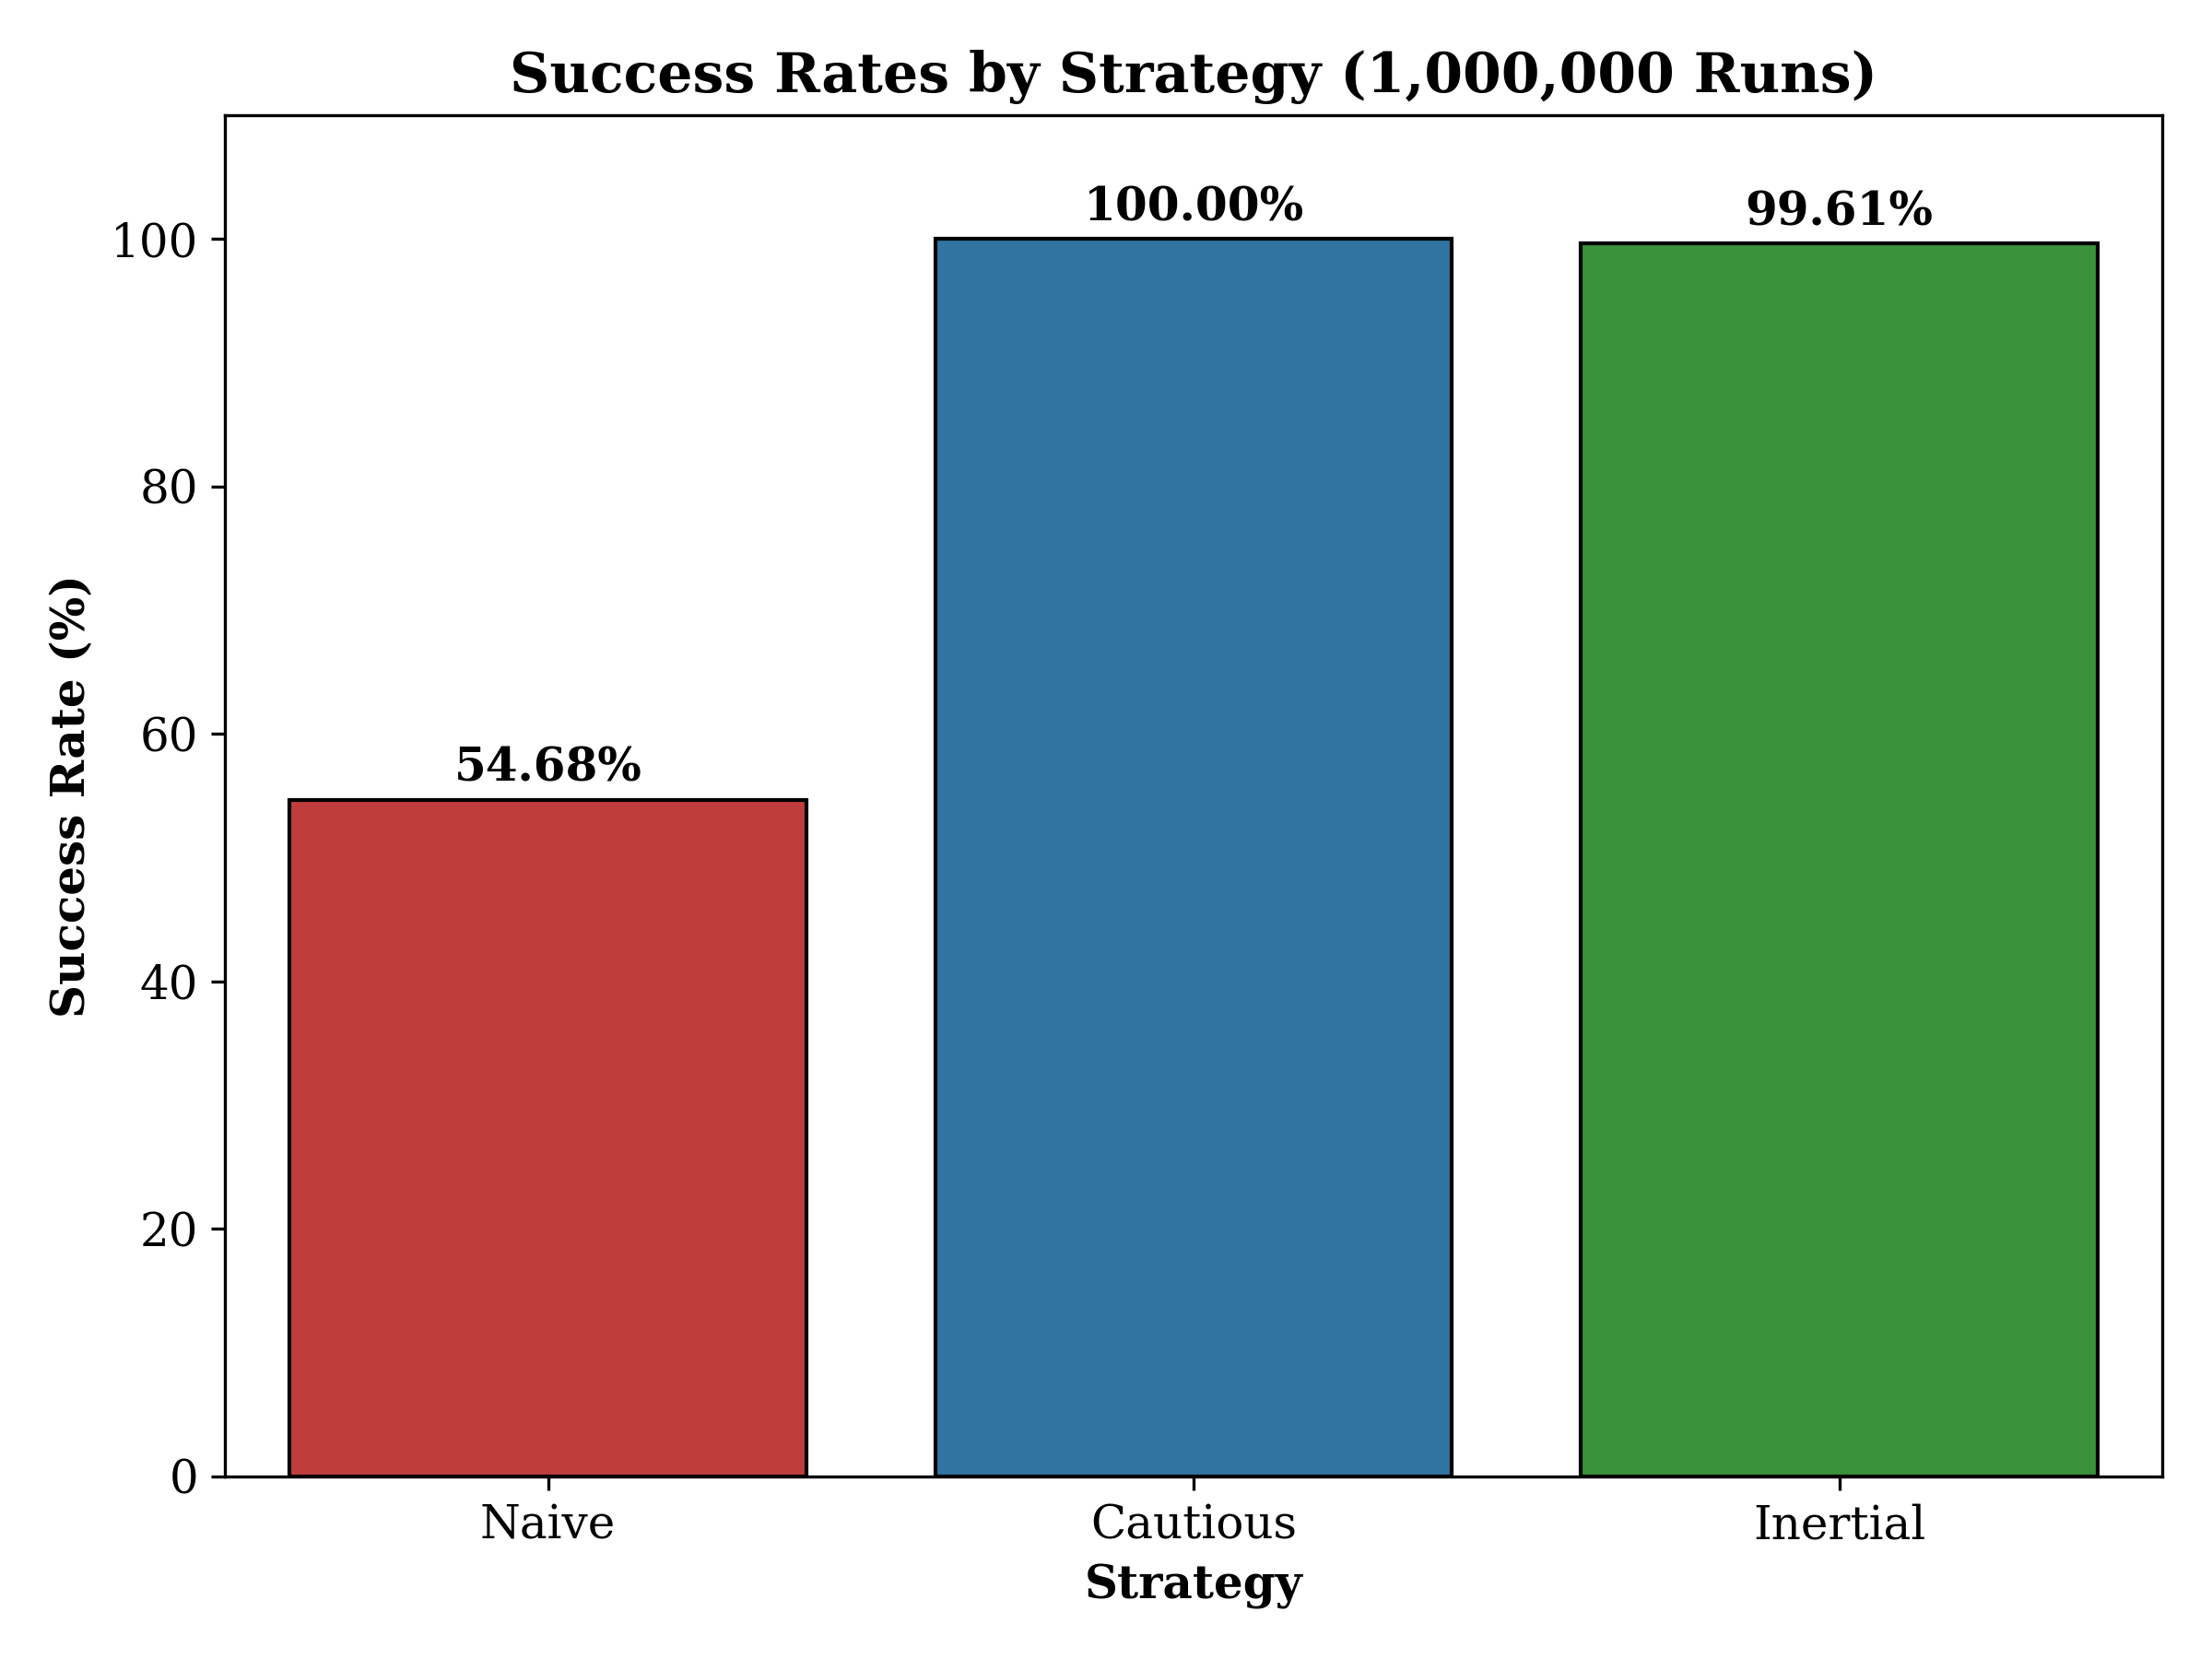
\includegraphics[width=0.85\linewidth]{success_rates.png}
    \caption{Success rates of the Naive, Cautious, and Inertial strategies across $1,000,000$ randomized superposition environments.}
    \label{fig:success_rates}
\end{figure}

As shown in Fig.~\ref{fig:success_rates} and Table~\ref{tab:efficiency}, the baseline \textit{Naive} strategy is severely compromised by additive superposition, succeeding in only $54.68\%$ of the sampled environments (failing in $45.32\%$ of cases), with representative failed trials exhibiting free-space gradient deflection ($u_{\text{ori}}$) under $\nabla_p S(p, t)$ and artificially inflated hit thresholds $i_H$ recorded during adversarial bursts that trap the robot in boundary-following loops. Even when the Naive strategy eventually reaches the target, adversarial gradient deflection inflates its mean trajectory duration to $199.3$ steps (and an unconditional horizon-capped mean of $\bar{N}_{\text{capped}} = 1015.4$ steps when failed runs are penalized at $N_{\max} = 2,000$).

\begin{table}[htbp]
\centering
\caption{Performance Comparison Under Superposition Spoofing ($1,000,000$ Paired Runs)}
\label{tab:efficiency}
\resizebox{\linewidth}{!}{%
\begin{tabular}{@{}lcccc@{}}
\toprule
\textbf{Strategy} & \textbf{Success Rate ($95\%$ CI)} & \textbf{Mean Steps (Succ.)} & \textbf{Median [IQR] (Succ.)} & \textbf{$\bar{N}_{\text{capped}}$ (All Runs)} \\ \midrule
\textit{Benign I-Bug (no attack)} & \textit{$100.00\%$} & \textit{$132.6$} & \textit{$126.0$ $[108.0,\, 150.0]$} & \textit{$132.6$} \\ \midrule
Naive (I-Bug \cite{taylor2014intensity}) & $54.68\% \pm 0.10\%$ & $199.3$ & $153.0$ $[121.0,\, 205.0]$ & $1015.4$ \\
Cautious (Proposed) & $\mathbf{100.00\%}$ ($[99.9996, 100]\%$) & $193.0$ & $178.0$ $[160.0,\, 215.0]$ & $193.0$ \\
Inertial (Proposed) & $99.61\% \pm 0.01\%$ & $\mathbf{153.4}$ & $\mathbf{135.0}$ $[115.0,\, 168.0]$ & $\mathbf{160.6}$ \\ \bottomrule
\end{tabular}%
}
\end{table}

In stark contrast, the \textit{Cautious} strategy achieved an observed $100.00\%$ success rate ($95\%$ Clopper--Pearson CI: $[99.9996\%, 100.00\%]$ under the sampled environment distribution) across all $1,000,000$ environments, corroborating Theorem~\ref{thm:cautious_convergence}. Because the no-attack benign I-Bug reference also succeeded in $100.00\%$ of the generated mazes (mean $132.6$ steps), this confirms \emph{trajectory and convergence preservation} rather than improvement over benign I-Bug: Cautious succeeded in every instance where benign I-Bug succeeded, satisfied the step bound of Eq.~\eqref{eq:step_bound} in all $1,000,000$ runs, and incurred a mean pausing overhead of $60.4$ steps ($+45.6\%$). By halting translational motion and locking internal memory throughout every detected spoofing burst, the Cautious robot isolates its control logic from the corrupted field. Theorem~\ref{thm:cautious_convergence} provides a finite execution bound relative to the corresponding benign completion time $N_{\text{ideal}}$; empirically, as seen in Fig.~\ref{fig:steps_dist}, Cautious exhibited a maximum observed completion time of $578$ steps ($\sim 580$ steps) across the one million sampled environments, whereas both the Naive and Inertial strategies exhibit long upper tails and large completion-time outliers extending up to the $2,000$-step horizon due to multi-orbit boundary trapping.

\begin{figure}[htbp]
    \centering
    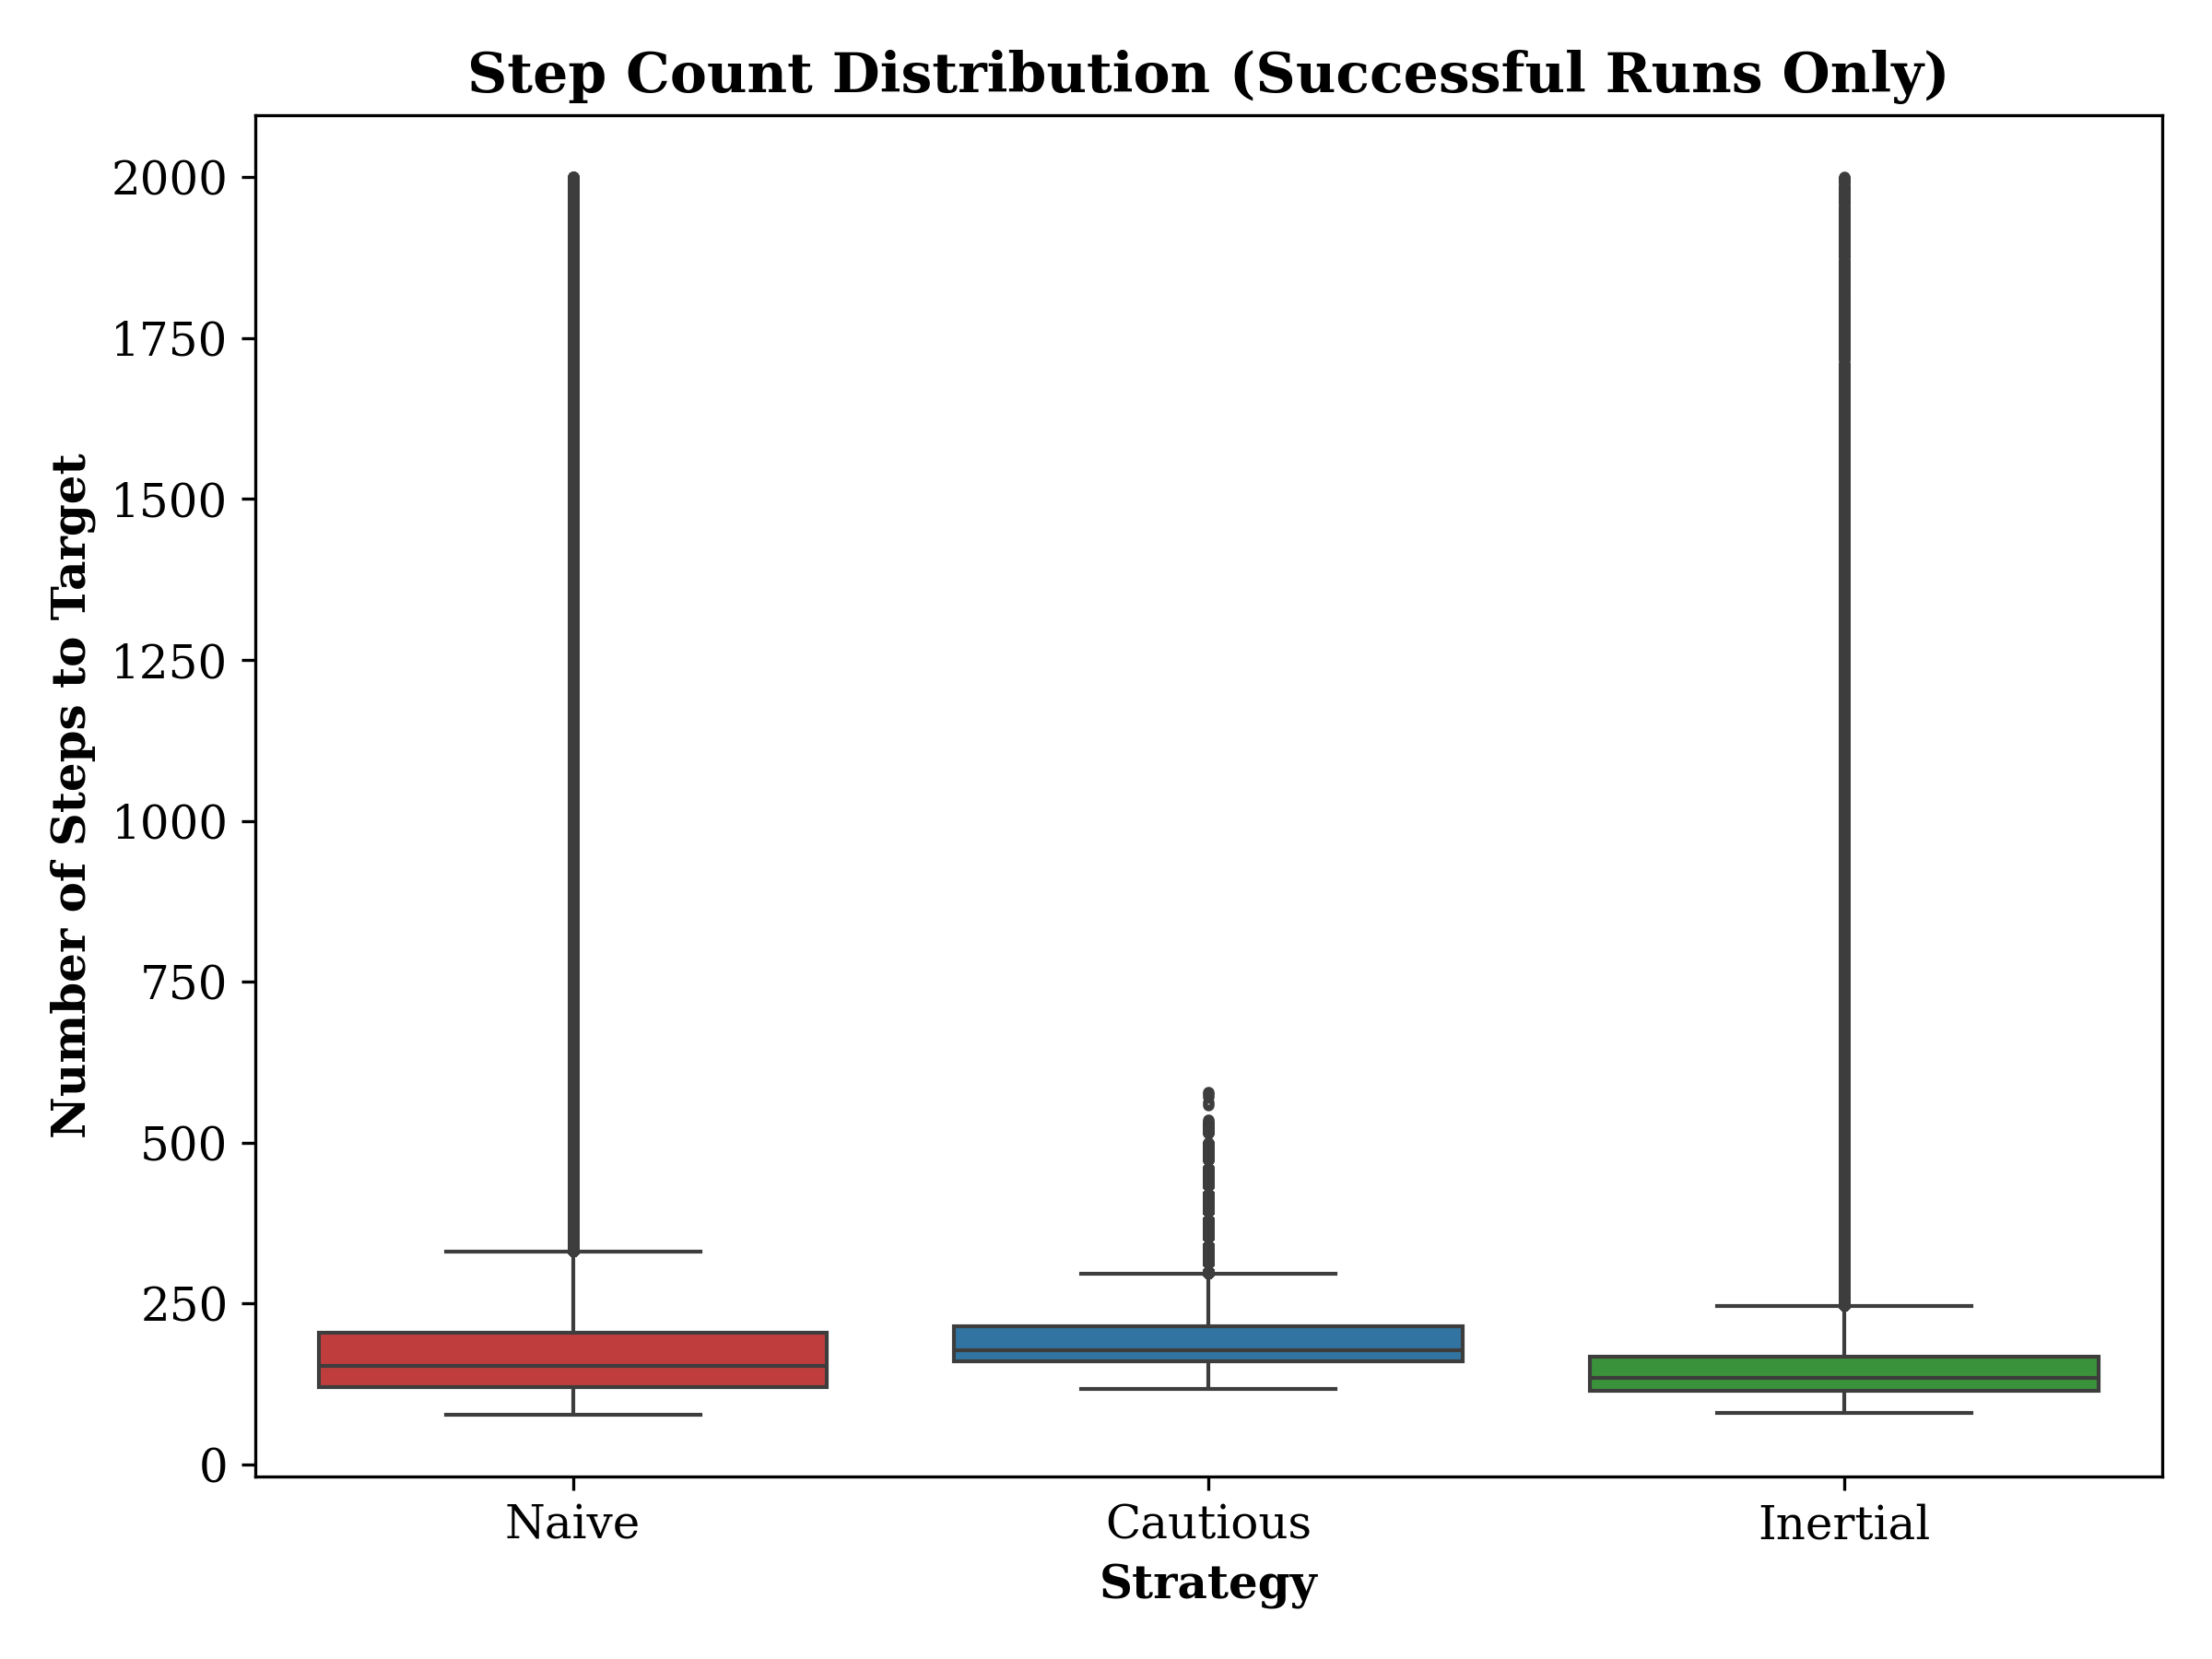
\includegraphics[width=0.85\linewidth]{steps_distribution.png}
    \caption{Distribution of step counts required to reach the target for successful runs. Across the $1,000,000$ sampled environments, the Cautious strategy exhibited a maximum observed completion time of $578$ steps ($\sim 580$) at the cost of a higher median due to adversarial pausing, whereas the Inertial heuristic minimizes average and median traversal duration among successful runs.}
    \label{fig:steps_dist}
\end{figure}

At the same time, Table~\ref{tab:efficiency} and Fig.~\ref{fig:steps_dist} highlight the operational trade-off of strict state preservation. Because the Cautious robot pauses for $T_{\text{on}} + N_{\text{confirm}} - 1 = 12$ steps per adversarial cycle, it requires an average of $193.0$ steps (median $178.0$) to reach the target. Conversely, among successful runs, the \textit{Inertial} heuristic reduces the mean completion step count to $153.4$ steps (median $135.0$)—a $20.5\%$ conditional reduction in mean steps ($24.2\%$ in median steps) relative to Cautious—while failing in $0.39\%$ of trials. Because conditioning on successful runs excludes the $3,877$ failed Inertial trials, Table~\ref{tab:efficiency} also reports the unconditional horizon-capped mission cost $\bar{N}_{\text{capped}} = \frac{1}{N}\sum_{j=1}^N \min(N_j, N_{\max})$, which penalizes failed trials at $N_{\max} = 2,000$. Under this risk-adjusted metric, Inertial averages $\bar{N}_{\text{capped}} = 160.6$ steps ($16.8\%$ lower than Cautious's $193.0$ steps), though any mission assigning a higher penalty to non-completion favors the Cautious strategy.

\subsection{Case Study: Cyclic Synchronization (Resonance) in the Inertial Strategy}
\label{subsec:resonance_case}
While the Inertial heuristic succeeds in $99.61\%$ of environments, its failure in the remaining $0.39\%$ ($3,877$ out of $1,000,000$ trials) is consistent with Proposition~\ref{prop:inertial_resonance}, and the following case study provides a concrete simulated instance of the proposed phase-locking mechanism.

\begin{figure}[htbp]
    \centering
    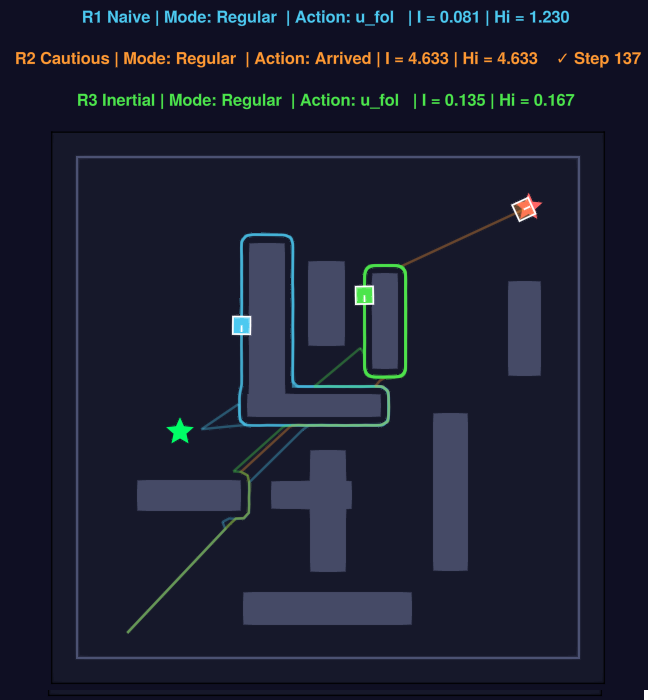
\includegraphics[width=0.8\linewidth]{simulation_trap.png}
    \caption{Visualization of a representative double-failure scenario. The Naive robot (cyan, $i_H = 1.230$) is permanently poisoned on the central L-shaped obstacle; the Inertial robot (green, $i_H = 0.167$) is caught in a Cyclic Synchronization (resonance) loop around the upper-right vertical obstacle because its passage across the top departure arc $\mathcal{A}_L$ repeatedly coincides with the $10$-step adversarial active window; the Cautious robot (orange) pauses during bursts and arrives at the target in $137$ steps.}
    \label{fig:sim_trap}
\end{figure}

Figure~\ref{fig:sim_trap} illustrates a representative trajectory from the simulation suite in which both the Naive and Inertial strategies fail via distinct mechanisms while the Cautious robot succeeds:
\begin{itemize}
    \item \textbf{Naive Poisoning:} The Naive robot (cyan) contacts the central L-shaped obstacle while the adversarial tower (green star) is broadcasting, recording a corrupted threshold $i_H = 1.230$ that exceeds the maximum legitimate target intensity anywhere along that obstacle boundary ($I \approx 0.081$), condemning it to orbit the L-obstacle indefinitely.
    \item \textbf{Inertial Cyclic Synchronization:} The Inertial robot (green) successfully clears the central obstacle with a valid threshold ($i_H = 0.167$) and contacts the upper-right vertical rectangular wall. However, the perimeter length of this rectangular obstacle induces an orbital period that phase-locks with the $40$-step adversarial cycle. Each time the Inertial robot approaches the top-right corner—the unique boundary departure arc $\mathcal{A}_L$ where $m(p - p_t) > 0.167$—the adversary activates for $10$ steps. Because peak detection is suspended during \texttt{InertialMode}, the robot rounds the top corner while blind and only resumes closed-loop sensing on the descending western face ($I = 0.135 < i_H$), locking it into a perpetual limit cycle.
    \item \textbf{Cautious Convergence:} The Cautious robot (orange) freezes on the boundary whenever the adversary activates, detects the true local maximum at the top-right corner once the burst subsides, departs toward the target beacon (red star), and arrives at step $137$.
\end{itemize}

\section{Limitations and Future Work}
\label{sec:limitations}
While our framework establishes a rigorous foundation for spoofing-resilient minimalist navigation, several practical extensions remain open for future investigation:

\begin{itemize}
    \item \textbf{Stochastic Sensor Noise and Multipath Fading:} Our anomaly detector relies on bounded deterministic spatial variations (Assumption~\ref{assump:discontinuity}). In physical RF or acoustic deployments, thermal noise and multipath fading introduce high-frequency stochastic fluctuations that could trigger false positives or mask small spoofing jumps. Future work will integrate sequential change-point detection (e.g., CUSUM \cite{basseville1993detection} or Kalman innovation filters) to separate adversarial shifts from zero-mean sensor noise.
    
    \item \textbf{Gradient-Ramping (Adiabatic) Attacks:} The detector exploits the step discontinuity of $u(t)$. An adaptive adversary that gradually ramps its transmission power $\alpha_e(t)$ at a rate $|\dot{\alpha}_e(t)|$ strictly below the robot's kinematic Lipschitz bound could evade temporal jump detection. Countering adiabatic spoofing within a minimalist sensor suite is an important open theoretical problem.
    
    \item \textbf{Stochastic Resonance-Breaking for the Inertial Heuristic:} Because Inertial trapping arises from deterministic phase-locking between $T_{\text{orbit}}$ and $T_{\text{cycle}}$ (Proposition~\ref{prop:inertial_resonance}), introducing randomized step-size jitter or brief stochastic pauses during \texttt{InertialMode} could break deterministic phase synchronization and potentially restore almost-sure convergence under suitable stochastic excitation assumptions while retaining most of the speed advantage of open-loop motion.
    
    \item \textbf{Mobile and Multi-Transmitter Adversaries:} Extending the framework to moving adversaries or coordinated multi-jammer networks with overlapping duty cycles requires generalizing the confirmation logic to track multi-level intensity steps.
    
    \item \textbf{Hardware Validation:} Building on the physical differential-drive validation of original I-Bug \cite{taylor2014intensity}, future work will deploy these algorithms on embedded mobile robots operating under real RF/optical interference.
\end{itemize}

\section{Conclusion}
\label{sec:conclusion}
This paper investigated the vulnerability of minimalist, intensity-based bug navigation algorithms to intermittent additive spoofing under an incoherent additive RSS superposition model. We demonstrated that without additional hardware, odometry, or localization, a robot can reliably detect adversarial interference by comparing temporal signal jumps against the local Lipschitz bounds dictated by its own kinematics.

We proved mathematically that under Assumptions~\ref{assump:superposition} and~\ref{assump:discontinuity}, the proposed \textit{Cautious} strategy conditionally preserves the exact active-state spatial trajectory and convergence guarantees of the underlying benign I-Bug execution, and corroborated this property across $1,000,000$ randomized simulation environments with an observed $100.00\%$ success rate (compared to $54.68\% \pm 0.10\%$ for the unmodified Naive I-Bug baseline). Furthermore, our evaluation of the open-loop \textit{Inertial} heuristic ($99.61\% \pm 0.01\%$ success rate, reducing mean steps among successful runs by $20.5\%$ and unconditional horizon-capped steps by $16.8\%$ relative to Cautious) demonstrated both its substantial average-case speed advantage and the theoretical insufficiency of memory freezing alone under topological phase-locking (Proposition~\ref{prop:inertial_resonance}). Together, these results provide a rigorous mathematical and empirical foundation for designing resilient, sensor-minimalist autonomous systems in contested environments.

\bibliographystyle{plain}
\begin{thebibliography}{10}

\bibitem{lumelsky1987path}
V.~J. Lumelsky and A.~A. Stepanov, ``Path-planning strategies for a point mobile automaton moving amidst unknown obstacles of arbitrary shape,'' \textit{Algorithmica}, vol.~2, no.~1, pp.~403--430, 1987.

\bibitem{kamon1998tangentbug}
I.~Kamon, E.~Rimon, and E.~Rivlin, ``TangentBug: A range-sensor-based navigation algorithm,'' \textit{Int. J. Robot. Res.}, vol.~17, no.~9, pp.~934--953, 1998.

\bibitem{taylor2009ibug}
K.~Taylor and S.~M. LaValle, ``I-Bug: An intensity-based bug algorithm,'' in \textit{Proc. IEEE Int. Conf. Robot. Autom. (ICRA)}, Kobe, Japan, 2009, pp.~3981--3986.

\bibitem{taylor2014intensity}
K.~Taylor and S.~M. LaValle, ``Intensity-based navigation with global guarantees,'' \textit{Autonomous Robots}, vol.~36, no.~4, pp.~349--364, 2014.

\bibitem{kerns2014unmanned}
A.~J. Kerns, D.~P. Shepard, J.~A. Bhatti, and T.~E. Humphreys, ``Unmanned aircraft capture and control via GPS spoofing,'' \textit{J. Field Robot.}, vol.~31, no.~4, pp.~617--636, 2014.

\bibitem{psiaki2016gnss}
M.~L. Psiaki and T.~E. Humphreys, ``GNSS spoofing and detection,'' \textit{Proc. IEEE}, vol.~104, no.~6, pp.~1258--1270, Jun. 2016.

\bibitem{pasqualetti2013attack}
F.~Pasqualetti, F.~D{\"o}rfler, and F.~Bullo, ``Attack detection and identification in cyber-physical systems,'' \textit{IEEE Trans. Autom. Control}, vol.~58, no.~11, pp.~2715--2729, Nov. 2013.

\bibitem{fawzi2014secure}
H.~Fawzi, P.~Tabuada, and S.~Diggavi, ``Secure estimation and control for cyber-physical systems under adversarial attacks,'' \textit{IEEE Trans. Autom. Control}, vol.~59, no.~6, pp.~1454--1467, Jun. 2014.

\bibitem{giraldo2018survey}
J.~Giraldo, D.~Urbina, A.~Cardenas, J.~Valente, M.~Faisal, J.~Ruths, N.~O. Tippenhauer, H.~Sandberg, and R.~Candell, ``A survey of physics-based attack detection in cyber-physical systems,'' \textit{ACM Comput. Surv.}, vol.~51, no.~4, Art.~no.~76, pp.~1--36, 2018.

\bibitem{basseville1993detection}
M.~Basseville and I.~V. Nikiforov, \textit{Detection of Abrupt Changes: Theory and Application}. Englewood Cliffs, NJ, USA: Prentice Hall, 1993.

\end{thebibliography}

\end{document}

